\chapter{Mathematics}

\section{Modular Arithmetic}

	\kactlimport{modular.cpp}

	\subsection{Lucas's Theorem}

	$$ \binom{n}{m} \equiv \prod_{i=0}^k \binom{n_i}{m_i} \quad (\text{mod } p) $$ 

	For $p$ prime. $n_i$ and $m_i$ are the coefficients of the representations of $n$ and $m$ in base $p$.

	\textit{Example:}

		11 (in base p=3) = $1 \cdot 3^2 + 0 \cdot 3^1 + 2 \cdot 3^0$

		$\implies n_2 = 1, n_1 = 0, n_0 = 2$

	\subsection{Fermat's Little Theorem}

	Fermat's little theorem states that if $p$ is a prime number, then for any integer $a$, the number $a^p - a$ is an integer multiple of $p$:

	$$ a^{p} \equiv a {\pmod {p}} $$

	If a is not divisible by p, that is, if a is coprime to p, then Fermat's little theorem is equivalent to:

	$$ a^{p-1} \equiv 1 {\pmod {p}} $$

	In other words, when doing a double exponentiation. Do:

	$$ a^{b^c} {\pmod {p}} \equiv a^{ ({b^c} {\pmod {p-1}}) } {\pmod {p}} $$

\section{Combinatorics}

	\begin{align*}
		\binom{n}{m} =  & \frac{ n! }{ m! \cdot (n-m)! }, & 0 <= m <= n \\
						& 0, & otherwise
	\end{align*}

	\subsection{Factorial}

		\begin{center}
			\begin{tabular}{l}
				\begin{tabular}{c|c@{\ }c@{\ }c@{\ }c@{\ }c@{\ }c@{\ }c@{\ }c@{\ }c@{\ }c}
				$n$  & 1 & 2 & 3 & 4  & 5   & 6   & 7    & 8     & 9      & 10\\
				\hline
				$n!$ & 1 & 2 & 6 & 24 & 120 & 720 & 5040 & 40320 & 362880 & 3628800\\
				\end{tabular}\\
				\begin{tabular}{c|c@{\ }c@{\ }c@{\ }c@{\ }c@{\ }c@{\ }c@{\ }c@{\ }c@{\ }c}
				$n$  & 11    & 12    & 13    & 14     & 15     & 16     & 17\\
				\hline
				$n!$ & 4.0e7 & 4.8e8 & 6.2e9 & 8.7e10 & 1.3e12 & 2.1e13 & 3.6e14\\
				\end{tabular}\\
				\begin{tabular}{c|c@{\ }c@{\ }c@{\ }c@{\ }c@{\ }c@{\ }c@{\ }c@{\ }c@{\ }c}
				$n$  & 20   & 25   & 30   & 40   & 50   & 100   & 150   & 171\\
				\hline
				$n!$ & 2e18 & 2e25 & 3e32 & 8e47 & 3e64 & 9e157 & 6e262 & \scriptsize{$>$DBL\_MAX}\\
				\end{tabular}
			\end{tabular}
		\end{center}

	\subsection{Combinatorial Struct}

		\kactlimport{combinatorics.cpp}

	\subsection{Burside Lemma}

	Let $G$ be a group that acts on a set $X$. The Burnside Lemma states that the number of distinct orbits is equal to the average number of points fixed by an element of G.
    $$T = \frac{1}{|G|} \sum_{g \in G} |\texttt{fix}(g)|$$
    Where a orbit $\texttt{orb}(x)$ is defined as
    $$\texttt{orb}(x) = \{y \in X : \exists g \in G \ gx = y \}$$
    and $\texttt{fix}(g)$ is the set of elements in $X$ fixed by $g$
    $$\texttt{fix}(g) = \{x \in X : gx = x\}$$
    
    \textbf{Example1:} With $k$ distinct types of beads how many distinct necklaces of size $n$ can be made? Considering that two necklaces are equal if the rotation of one gives the other.
    
	\begin{center}
    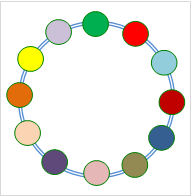
\includegraphics[scale=.6, keepaspectratio]{content/math/Burnside-Necklace.png}
    \end{center}
	$$\frac{1}{n} \sum_{i=1}^n k^{\gcd(i, n)}$$

	\textbf{Example2:} Count the number of different n $\times$ n grids whose each square is black or white.

	Two grids are considered to be different if it is not possible to rotate one of them so that they look the same.
	
	\begin{center}
	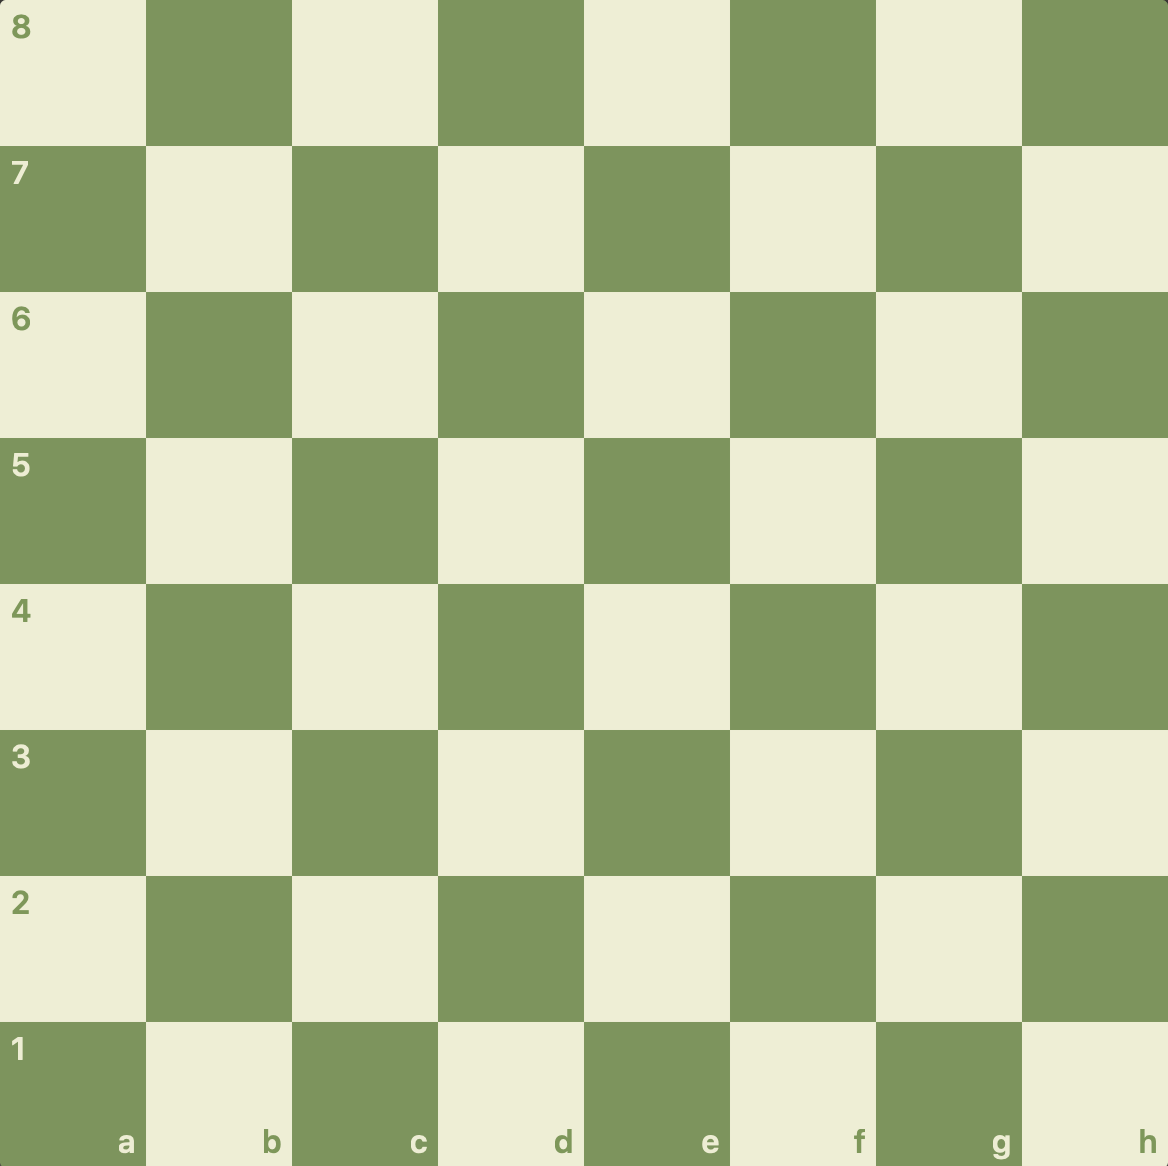
\includegraphics[scale=.1, keepaspectratio]{content/math/Burnside-Grid.png}
	\end{center}

	$$ G (Rotations) = 0^{\circ}, 90^{\circ}, 180^{\circ}, 270^{\circ} $$

	\begin{centering}
	\begin{align*}
	f(rotation) = & \\
	0^{\circ}: 				& 2^{(n^2)}  \\
	90^{\circ}/270^{\circ}:	& 2^{ \frac{n^2}{4} }, & n_{even} \\
							& 2^{ \frac{n^2-1}{4} } \cdot 2 , & n_{odd} \\
	180^{\circ}:			& 2^{ \frac{n^2}{2} }, & n_{even} \\
							& 2^{ \frac{n^2-1}{2} } \cdot 2 , & n_{odd}
	\end{align*}
	\end{centering}

	
	$$ans = \frac{1}{4} (f(0^{\circ}) + f(90^{\circ}) + f(180^{\circ}) + f(270^{\circ})) $$

	\subsection{Interesting Recursion}

	$$ f(a, b) = f(a-1, b) + f(a, b-1) $$

	$$ \implies f(a, b) = \frac{(a+b)!}{a! b!} = \binom{a+b}{a} $$

	\textit{Proof:}
	
	\begin{align*}
	&f(a, b) = \frac{(a+b)!}{a! b!}  \\ 
	\implies &f(a-1, b) = \frac{(a-1+b)!}{(a-1)! b!}, f(a, b-1) = \frac{(a+b-1)!}{a! (b-1)!}  \\
	\implies &f(a-1, b) + f(a, b-1) = \frac{(a-1+b)!}{(a-1)! b!} + \frac{(a+b-1)!}{a! (b-1)!}  \\
	\implies &f(a, b) = (a+b-1)! \cdot ( \frac{1}{(a-1)!(b)!} + \frac{1}{(a)!(b-1)!} )  \\
	\implies &f(a, b) = (a+b-1)! \cdot ( \frac{a+b}{a! b!} ) \\
	\implies &f(a, b) = \frac{(a+b)!}{a! b!} = \binom{a+b}{a} 
	\end{align*}

	\subsection{Couting Bishops}

	\kactlimport{bishops.cpp}




\section{Number Theory}

\subsection{Highly Composite Numbers}

	\begin{center}
		\footnotesize
		\begin{tabular}{|c|r|r|l|}
		\hline
		\textbf{\textless{}=} & \multicolumn{1}{c|}{\textbf{Divisors}} & \multicolumn{1}{c|}{\textbf{Number}} & \multicolumn{1}{c|}{\textbf{Factorization}} \\ \hline
		1e3                 & 32                                     & 840                                  & $ 2^3 \thinspace 3   \thinspace 5   \thinspace 7                                   $ \\ \hline
		1e4                 & 64                                     & 7560                                 & $ 2^3 \thinspace 3^3 \thinspace 5   \thinspace 7                                 $ \\ \hline
		1e5                 & 128                                    & 83160                                & $ 2^3 \thinspace 3^3 \thinspace 5   \thinspace 7   \thinspace 11                              $ \\ \hline
		1e6                 & 240                                    & 720720                               & $ 2^4 \thinspace 3^2 \thinspace 5   \thinspace 7   \thinspace 11 \thinspace 13                           $ \\ \hline
		1e9                 & 1344                                   & 735134400                            & $ 2^6 \thinspace 3^3 \thinspace 5^2 \thinspace 7   \thinspace 11 \thinspace 13 \thinspace 17                      $ \\ \hline
		1e12                & 6720                                   & 963761198400                         & $ 2^6 \thinspace 3^4 \thinspace 5^2 \thinspace 7   \thinspace 11 \thinspace 13 \thinspace 17 \thinspace 19 \thinspace 23                $ \\ \hline
		1e14                & 17280                                  & 97821761637600                       & $ 2^5 \thinspace 3^4 \thinspace 5^2 \thinspace 7^2 \thinspace 11 \thinspace 13 \thinspace 17 \thinspace 19 \thinspace 23 \thinspace 29           $ \\ \hline
		1e15                & 26880                                  & 866421317361600                      & $ 2^6 \thinspace 3^4 \thinspace 5^2 \thinspace 7   \thinspace 11 \thinspace 13 \thinspace 17 \thinspace 19 \thinspace 23 \thinspace 29 \thinspace 31          $ \\ \hline
		1e18                & 103680                                 & 897612484786617600                   & $ 2^8 \thinspace 3^4 \thinspace 5^2 \thinspace 7^2 \thinspace 11 \thinspace 13 \thinspace 17 \thinspace 19 \thinspace 23 \thinspace 29 \thinspace 31 \thinspace 37     $ \\ \hline
		\end{tabular}
	\end{center}

\subsection{Divisibility}
	
	``a is divisible by b'' or
	``a is a multiple of b'' or
	``b is a divisor of a'' or
	``b is a factor of a'' or
	``b divides a'' or
	``$(b | a)$''

	$$ a \% b == 0 $$

	``a1, a2 are divisible by b''
	$$ gcd(a1, a2) \% b = 0 $$

	``a is divisible by b1 and b2''
	$$ a \% lcm(b1, b2) = 0 $$
	
	\subsubsection{Euclid}
	$$ a = bq + r $$

	\subsubsection{Lema 1 - Transitivity}

	``a is divisible by b and b is divisible by c''

	$$ (a | b) , (b | c)  \implies (a | c) $$

	\subsubsection{Lema 2}
	$$ (a | b) , (a | c) => a | (rb + sc) $$

	\subsubsection{Lema 3}
	$$ d = gcd(a, b) \implies gcd(a/d, b/d) = 1 $$

	\subsubsection{Lema 4}
	$$ d = gcd(a, b) \implies d = ra + sb \implies (d_0 | a), (d_0 | b) \implies (d_0 | d) $$
	
	\subsubsection{Lema 5}
	$$ (a | bc), gcd(a, b) = 1 \implies (a | c) $$

	\subsubsection{Lema 6}
	$$ a = bq+r, {1 <= r < b} \implies gcd(a, b) = gcd(b, r) $$
	
	\subsubsection{Greatest Common Divisor (GCD)}
	
		$$ gcd(a) = a $$
		$$ gcd(a, b, c) = gcd( gcd(a, b), c ) $$ 
		$$ gcd(a, b) = (a*b) / lcm(a, b) $$
	
	\subsubsection{Least Commom Multiple (LCM)}
	
		$$ lcm(a) = a $$
		$$ lcm(a, b, c) = lcm( lcm(a, b), c ) $$
		$$ lcm(a, b) = (a*b) / gcd(a, b) $$
	
	\textbf{Observation:} \textit{std-c++17} implements $gcd()$ function, which works correctly for negative numbers as well:
	
	$$ gcd(a,b) = gcd(-a,-b) = gcd(-a,b) = gcd(a,-b) $$
	
\subsection{Closed Formulas related to divisors of a number}
	
	Let $n$ be a number represented by it's prime factors $p_i$ and respective exponents $e_i$:
	
	$$ n = p_1^{e_1} \cdot p_2^{e_2} \cdots p_k^{e_k} $$
	
	\subsubsection{Number of Divisors}
	
	$$ d(n) = (e_1 + 1) \cdot (e_2 + 1) \cdots (e_k + 1) $$
	$$ C_i = C_{i-1} \cdot (e_i + 1) $$
	
	\subsubsection{Sum of Divisors}
	
	$$ \sigma(n) = \frac{p_1^{e_1 + 1} - 1}{p_1 - 1} \cdot \frac{p_2^{e_2 + 1} - 1}{p_2 - 1} \cdots \frac{p_k^{e_k + 1} - 1}{p_k - 1} $$
	
	$$ S_i = S_{i-1} \cdot \frac{p_i^{e_i + i} - 1}{p_i - 1} $$
	
	\subsubsection{Product of Divisors}
	
	$$ P_i = (P_{i-1})^{(e_i + 1)} \cdot ({p_i}^{(e_i(e_i + 1))/2})^{C_{i-1}} $$
	
	where, $ C_i = $ ``Number of Divisors considering $i$ factors''.
	And remeber to use \textbf{Fermat's Little Theorem}
	
\subsection{Sieves}
	
	These sieves are used to find all primes up to an upper bound N, which is usually $10^7$

	\subsubsection{Eratosthenes}

		Eratosthenes uses less memory than the linear sieve and is almost as fast

		\kactlimport{eratosthenes.cpp}

	\subsubsection{Linear Sieve}

		Due to the lp vector, one can compute the factorization of any number very quickly!

		Can check primality with $lp[i] == i$

		Uses more memory, because lp is a vector of int or ll and not bits.

		\textbf{Proof of time complexity:}

		We need to prove that the algorithm sets all values
		$lp[]$ correctly, and that every value will be set exactly once. 
		Hence, the algorithm will have linear runtime, since all the remaining actions of the algorithm, obviously, work for
		$O(n)$.

		Notice that every number $i$ has exactly one representation in form:
		$$i = lp [i] \cdot x,$$
		where 
		$lp [i]$ is the minimal prime factor of 
		$i$, and the number 
		$x$ doesn't have any prime factors less than 
		$lp [i]$, i.e.
		$$lp [i] \le lp [x].$$
		Now, let's compare this with the actions of our algorithm: in fact, for every 
		$x$ it goes through all prime numbers it could be multiplied by, i.e. all prime numbers up to 
		$lp [x]$ inclusive, in order to get the numbers in the form given above.

		Hence, the algorithm will go through every composite number exactly once, setting the correct values 
		$lp []$ there. Q.E.D.

		\kactlimport{linear-sieve.cpp}
	
\subsection{Extended Euclid}
	
	Solves the $ ax + by = gcd(a, b)$ equation.

	\subsubsection{Inverse Multiplicative}

	if \textbf{ $gcd(a, b) = 1$ }:

	then:

	$$ax + by \equiv 1$$

	also, if you apply $\pmod{b}$ to the equation:

	$$ ax \pmod{b} + by \pmod{b} \equiv 1 \pmod{b} $$
	$$ ax \equiv 1 \pmod{b} $$

	In other words, one can find the inverse multiplicative of any number $a$ in modulo $b$ if $gcd(a, b) = 1$

	\subsubsection{Diofantine Equation}

	$$ ax \equiv c \pmod{b} $$

	if $g = gcd({a, b, c}) \neq 1$, divide everything by $g$.

	After this, if $gcd(a, b) = 1$, find $a^{-1}$, then multiply both sides of the Diofantine equation.

	$$ x \equiv c * a^{-1} \pmod{b} $$

	After this, one has simply found $x$

	\kactlimport{extended-euclid.cpp}


\section{FFT}

	FFT can be used to turn a polynomial multiplication complexity to $O(N \log{N})$.

	A \textbf{convulution} is easily computed by inverting the second vector and doing the polynomial multiplication normally.

	\kactlimport{fft-simple.cpp}

\section{Matrix}

For faster linear recurrence computation with matrix exponentiation. 

$$ Base * Operator^{k} = Result $$

\kactlimport{matrix.cpp}

\subsection{Minimum Path Length with exactly k edges}

Consider a directed weighted graph having $n$ nodes and $m$ edges.
Your task is to calculate the minimum path length from node $1$ to node $n$ with exactly $k$ edges.

This task is solved the using matrix exponentiation the 
same way as the problem of \textbf{Counting the Number of Paths with exactly k edges}.
But there are some modifications in the matrix properties: 

The $null$ (and default) element is now $INF$. The identity is composed of $0$ in the diagonal.
And the product of matrices defined as:

$$ AB[i, j] = \min^{n}_{k=1} (AB[i, j], A[i,k] + B[k, j]) $$

Finally, the operator matrix contains the value of the minimum weight in each pairwise nodes or $INF$ (if no edges). 

\section{Series' Closed Formulas}

\subsection{Natural Number Summation (PA)}

$$ 1 + 2 + 3 + 4 + 5 + ... + n-1 + n $$
$$ = \sum_{i=1}^n i = \frac{ n(n+1) }{ 2 } $$

\subsection{Natural Number Quadratic Summation}

$$ 1 + 4 + 9 + 16 + 25 + ... + (n-1)^2 + n^2 $$
$$ = \sum_{i=1}^n i^2 = \frac{ n(n+1)(2n+1) }{ 6 } $$

\subsection{Triangular Numbers Summation}

$$ 1 + 3 + 6 + 10 + 15 + ... + \frac{(n-1)(n)}{2} + \frac{(n)(n+1)}{2} $$
$$ = \sum_{i=1}^n \frac{i(i+1)}{2} = \frac{1}{2}(\sum_{i=1}^n i^2 + \sum_{i=1}^n i) $$
$$ = \frac{1}{2} ( \frac{ n(n+1) }{ 2 } + \frac{ n(n+1)(2n+1) }{ 6 }) $$